\chapter{PNb data analysis}
\label{chapter:analysis_pNb}
Complemantary to data from pp exeriment data collected during pNb experiment was analized. Main scope of the studies was the same, aldough differences in collided system has forced some minnor changes in analysis methods. As a result inclusive \css for $\Ls$ together with the reference state $\Lz \Kz$ were measured and compared to the previous HADES studies \cite{hades_Sz_pNb,hades_Lp_femtoscopy_pNb,hades_arnold_pNb,hades_Ksi_pNb}. It allows to extend knowladge about hyperons into a pNb reactions and to point key diffrences between proton-proton and pronon-nucleon reactions.

\section{Data from pNb experiment}
The p(3.5 GeV) +Nb  experiemnt took place in October 2008. The beam with kinetic energy 3.5 GeV was delivered by the SIS 18 synchrotron and aimed into a segmented, 12-fold target. The target fickness was adjusted to get a 2.8\% interaction probability. The trigger system was the same as for pp@3.5 GeV experiment with LVL1 trigger based on hits multiplicity in META detector and LVL2 trigger dedicated for di-lepton studies. During experiment an avrege beam intensity was $2 \times 10^6$ particles/s, what gave in total $3.2 \times 10^9$ LVL1 events recorded on tapes.  


\section{Identyfication and data selection}
Identyfication and selection algorithms used for pNb data were the same as in case of a pp data analaysis. However in proton-nucleus reaction it is impossible to directly use the energy-momentum conservation rule. They are two main obstacles: part of four-momentum may be transfered to the nucleus as a recoil and nuceons in nucleus are not in rest. All together prevents from a use of the missing mass cut. The missing mass spectrum, in contrary to pp data, does not have any resosnans behavour. As a replacement a set of more restricted hurd cuts was applayed for  $\Lz$ reconstruction.
\begin{figure}
  \centering
  \caption{The missing mass spectrum for $\p \pim \pip \pim$ hypothesis.}
  \label{fig:miss_mass_pNb}
\end{figure}

\section{The $\Lz$ Reconstruction}
The main tool for $\Lz$ reconstruction stays the same as for in chapter \ref{chapter:analysis}. It is a neural network trained in a data-driven maner. Aldouth for a good signal extraction a set of additional pre-cuts was necessary. They are summerized in tab. ???

After applaying all cuts described in above table a signal~to~background ratio ??? was obtained. The result is shown in fig. \ref{fig:L1116SB_pNb}.
\begin{figure}[ht]
  \centering
  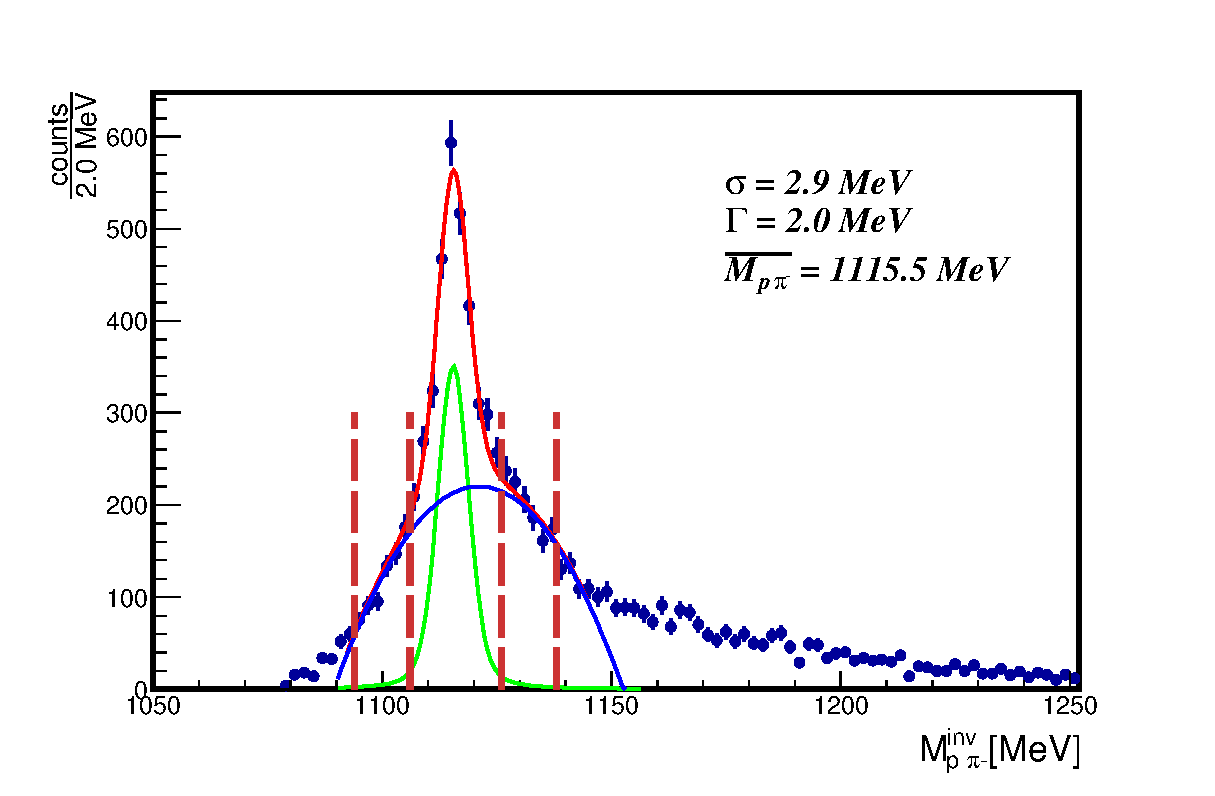
\includegraphics[width=0.7 \linewidth]{Chapter_analysisPNb/Lz.eps}
  \caption{The $\Lz$ spectrum after a neural network analysis obtained for pNb experiment. Color coding the same as in fig. \ref{fig:L1116SB}, vertical lines denotes regions of a side-band and were adjusted for pNb exclusively.}
  \label{fig:L1116SB_pNb}
\end{figure}

\section{The $\Lz \Kz $reconstruction}
The same as for in case of pp data an inclusive $\Lz \Kz$ production was a cross-check for en event selection method and absolute normalization. The rormalization method used for a \cs extraction was the same like described in \ref{sec:normalization} with two quantitive differences. The first: a total luminocity for pN experoiment was ???, the second: a knowledge about inclusive \css for proton-nucleus scattering is strongly limmited. Instead of exact values the universal scaling between reaction was asssumed:
\begin{equation}
  \sigma_{pN}=\sigma_{pp} \cdot A^{2/3}
\end{equation}

The obtained results gives well description for signals extracted from experimental data-set. 

\begin{figure}[ht]
  \centering
  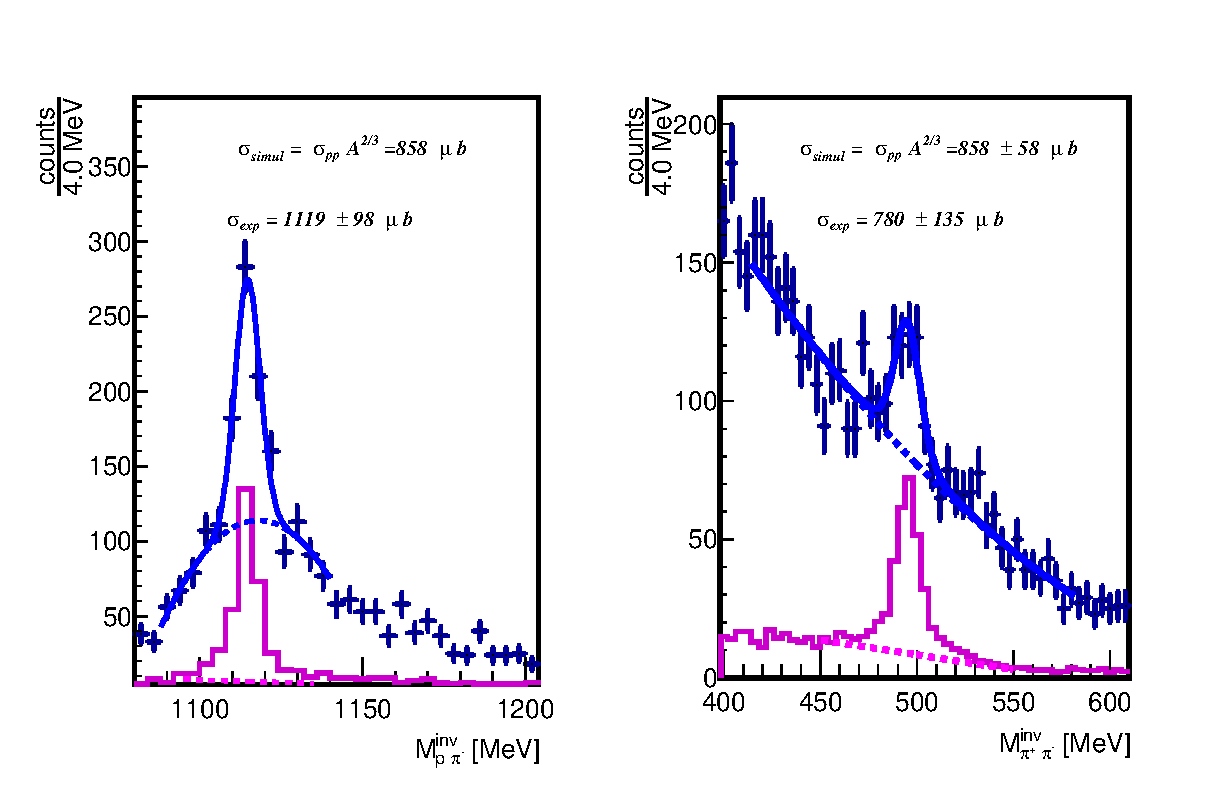
\includegraphics[width=0.9 \linewidth]{Chapter_analysisPNb/LK0.eps}
  \caption{The inclusive $\Lz \Kz$ spectrum obtained for pNb experiment. The \css for the simulation was scaled up by a factor $A^{2/3}$ compare values measured in pp reactions}
  \label{fig:LK0_pNb}
\end{figure}

\section{The $\Ls$ Reconstruction}



\subsection{Event mixing}


\subsection{Cross-section and extraction differential analysis}
\begin{figure}[ht]
  \centering
  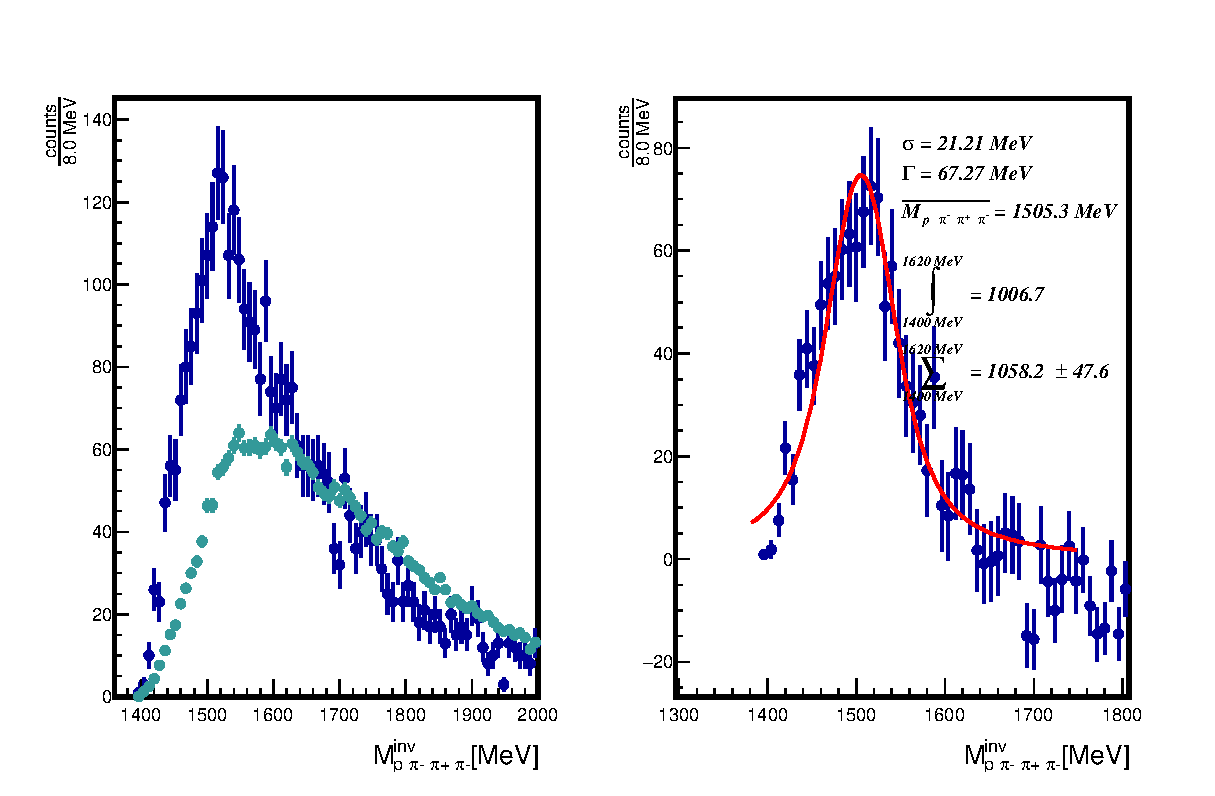
\includegraphics[width=0.9 \linewidth]{Chapter_analysisPNb/L1520.eps}
  \caption{a}
  \label{fig:L1520_pNb}
\end{figure}

\begin{figure}[ht]
  \centering
  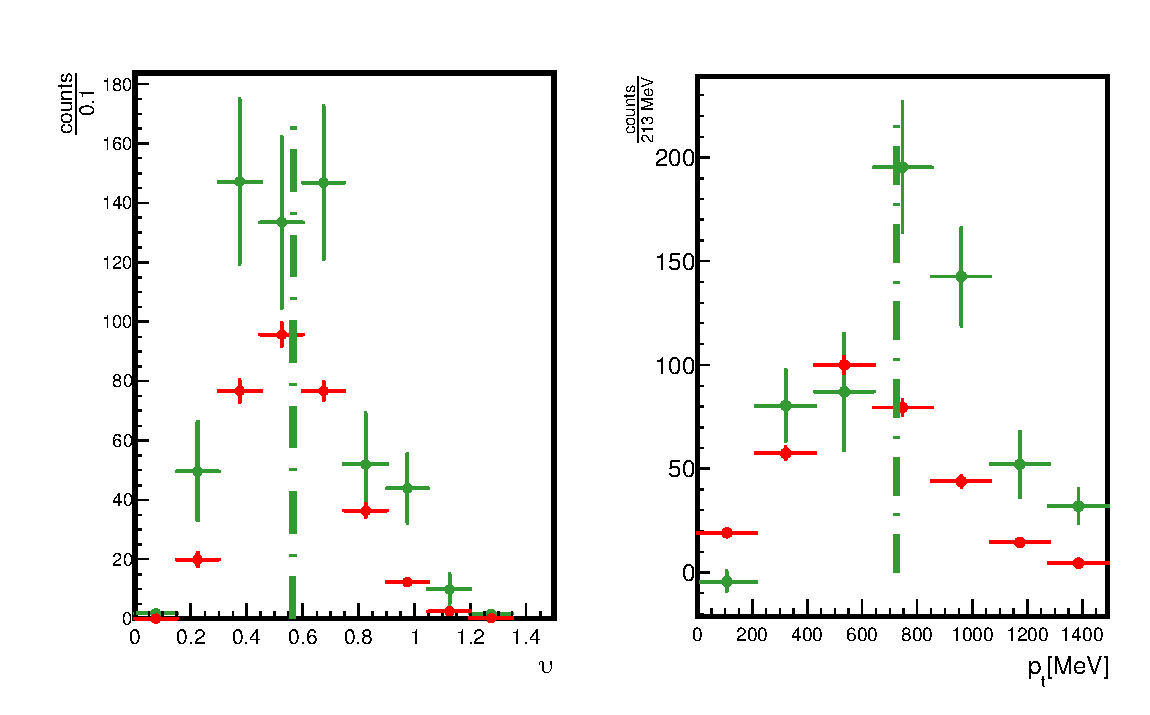
\includegraphics[width=0.9 \linewidth]{Chapter_analysisPNb/YPt.eps}
  \caption{b}
  \label{fig:YPt_pNb}
\end{figure}

\section{Comparison with results from pp data}